\chapter{Listarakenteet}

Lista on tietorakenne, joka sisältää joukon alkioita tietyssä järjestyksessä.
Esimerkiksi $[3,7,2,5]$ on lista, jossa on neljä alkiota.
Tavoitteemme on, että voimme tehokkaasti lisätä ja poistaa listan alkioita.

Tämä luku käsittelee kaksi tapaa listan toteuttamiseen:

\begin{itemize}
\item \textbf{Taulukkolista}: Lista on toteutettu taulukkona,
jonka kokoa muutetaan tarvittaessa.
\item \textbf{Linkitetty lista}: Lista on toteutettu erillisinä solmuina,
jotka on linkitetty toisiinsa.
\end{itemize}

Molemmissa toteutuksissa on omat hyvät ja huonot puolensa,
joihin kiinnitämme huomiota luvun aikana.

\section{Taulukkolista}

Taulukko on tehokas perustietorakenne, joka soveltuu hyvin listan alustaksi.
Ainoa ongelma on, että taulukon koko on kiinteä: meidän täytyy päättää alussa,
montako alkiota taulukossa on, emmekä voi muuttaa kokoa myöhemmin.
Esimerkiksi seuraava koodi luo taulukon, jossa on 10 alkiota:

\begin{code}
int[] taulu = new int[10];
\end{code}

Kuinka voisimme luoda muuttuvan kokoisen listan taulukon avulla?
Ratkaisuna on, että varaamme taulukkoon \emph{ylimääräistä}
tilaa tuleville listan alkioille.
Tälla tavalla voimme luoda listan, joka pystyy laajentumaan.
Seuraavaksi käymme läpi kaksi toteutusta,
joista ensimmäisessä listan loppuun voi lisätä alkioita
ja toisessa sekä alkuun että loppuun voi lisätä alkioita.

\subsection{Lisääminen loppuun}

Ideana on säilyttää listaa taulukossa niin,
että tietty määrä taulukon ensimmäisiä alkioita on listan käytössä
ja loput alkiot on varattu tuleville alkioille.
Kuva \ref{fig:listau} näyttää esimerkin listan $[3,7,2,5]$ tallentamisesta taulukkoon.
Taulukossa on paikkoja kymmenelle alkiolle, ja niistä neljä on tällä hetkellä käytössä.
Kun listan loppuun lisätään uusi alkio 6, se mahtuu taulukkoon.
Tällä tavalla alkion lisääminen listaan vie vain $O(1)$ aikaa.

\begin{figure}
\center
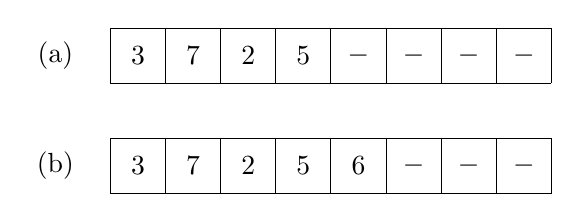
\begin{tikzpicture}[scale=0.7]
\begin{scope}
\draw (0,0) grid (8,1);
\node at (-1,0.5) {(a)};
\node at (0.5,0.5) {$3$};
\node at (1.5,0.5) {$7$};
\node at (2.5,0.5) {$2$};
\node at (3.5,0.5) {$5$};
\node at (4.5,0.5) {$-$};
\node at (5.5,0.5) {$-$};
\node at (6.5,0.5) {$-$};
\node at (7.5,0.5) {$-$};
\end{scope}
\begin{scope}[yshift=-2cm]
\draw (0,0) grid (8,1);
\node at (-1,0.5) {(b)};
\node at (0.5,0.5) {$3$};
\node at (1.5,0.5) {$7$};
\node at (2.5,0.5) {$2$};
\node at (3.5,0.5) {$5$};
\node at (4.5,0.5) {$6$};
\node at (5.5,0.5) {$-$};
\node at (6.5,0.5) {$-$};
\node at (7.5,0.5) {$-$};
\end{scope}
\end{tikzpicture}
\caption{(a) Lista $[3,7,2,5]$ tallennettuna taulukkoon. (b) Listan loppuun lisätään alkio 6.}
\label{fig:listau}
\end{figure}

Tässä on kuitenkin yksi ongelma: jossain vaiheessa koko taulukko
voi täyttyä eikä uusi listalle lisättävä alkio mahdu enää taulukkoon.
Kuva \ref{fig:lisuus} näyttää tällaisen tilanteen,
jossa uusi alkio 4 ei mahdu taulukkoon.
Tällöin meidän täytyy varata uusi suurempi taulukko ja
kopioida kaikki vanhan listan alkiot siihen.
Joudumme siis tekemään jotain seuraavanlaista,
jossa $n$ on taulukon nykyinen koko ja $k$ on varattavien
lisäpaikkojen määrä.

\begin{code}
int[] uusi = new int[n+k];
for (int i = 0; i < n; i++) {
    uusi[i] = lista[i];
}
lista = uusi;
\end{code}

Tämä on hidas operaatio, johon kuluu aikaa $O(n)$.
Olemme saaneet siis aikaan listan, johon on \emph{yleensä} nopeaa lisätä
alkioita, mutta välillä lisääminen viekin aikaa $O(n)$
uuden taulukon varaamisen ja kopioinnin takia.

\begin{figure}
\center
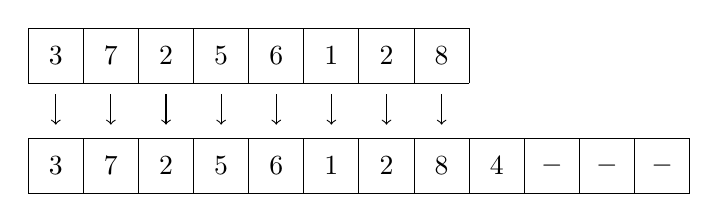
\begin{tikzpicture}[scale=0.7]
\begin{scope}
\draw (0,0) grid (8,1);
\node at (0.5,0.5) {$3$};
\node at (1.5,0.5) {$7$};
\node at (2.5,0.5) {$2$};
\node at (3.5,0.5) {$5$};
\node at (4.5,0.5) {$6$};
\node at (5.5,0.5) {$1$};
\node at (6.5,0.5) {$2$};
\node at (7.5,0.5) {$8$};
\foreach \x in {0,...,7} \draw[->] (\x+0.5,-0.2) -- (\x+0.5,-0.75);
\end{scope}
\begin{scope}[yshift=-2cm]
\draw (0,0) grid (12,1);
\node at (0.5,0.5) {$3$};
\node at (1.5,0.5) {$7$};
\node at (2.5,0.5) {$2$};
\node at (3.5,0.5) {$5$};
\node at (4.5,0.5) {$6$};
\node at (5.5,0.5) {$1$};
\node at (6.5,0.5) {$2$};
\node at (7.5,0.5) {$8$};
\node at (8.5,0.5) {$4$};
\node at (9.5,0.5) {$-$};
\node at (10.5,0.5) {$-$};
\node at (11.5,0.5) {$-$};
\end{scope}
\end{tikzpicture}
\caption{Taulukkoon ei mahdu enää uutta alkiota. Meidän täytyy varata uusi suurempi taulukko
ja kopioida vanhan taulukon sisältö sinne.}
\label{fig:lisuus}
\end{figure}

Jotta rakenne olisi käyttökelpoinen, meidän täytyy varmistaa,
että hidas $O(n)$-operaatio ei esiinny liian usein.
Tämä on mahdollista, kun varaamme uuden taulukon aina reilusti aiempaa suuremmaksi.
Tyypillinen tapa on varata uusi taulukko niin,
että sen koko on kaksinkertainen vanhaan taulukkoon nähden.
Kun toimimme näin, jokaisen alkion lisääminen listalle vie
\emph{keskimäärin} vain $O(1)$ aikaa.

Voimme ajatella asian näin: jokainen listalle lisättävä alkio
maksaa pääsy\-maksuna kolme euroa.
Tästä yksi euro menee listalle liittymiseen ja kaksi euroa jäävät säästöön.
Sitten kun aikanaan listalle täytyy varata suurempi taulukko,
jokainen viime erässä lisätty alkio maksaa yhden euron omasta siirrostaan
ja yhden euron aiemmin lisätyn alkion siirrosta.
Koska taulukon koko kaksinkertaistuu joka vaiheessa,
kolmen euron kiinteä pääsymaksu riittää siihen, että kaikki tulevat
siirrot saadaan kustannettua.

Miksi sitten emme voisi varata heti aluksi niin suurta taulukkoa,
että lopullinen lista mahtuisi siihen varmasti?
Tässä tulisi ongelmaksi, että listamme tuhlaisi paljon muistia.
Ohjelmassa saattaa olla samaan aikaan käytössä monia listoja,
ja haluamme, että listan varaama taulukko on samaa kokoluokkaa
kuin listan todellinen sisältö.

\subsection{Lisääminen alkuun ja loppuun}

Vastaavasti voimme luoda taulukkoon perustuvan listan,
johon voimme lisätä alkioita tehokkaasti sekä alkuun että loppuun.
Voimme menetellä lähes samoin kuin ennenkin,
kunhan luovumme yhdestä periaatteesta:
taulukon ensimmäinen alkio ei enää välttämättä
ole listan ensimmäinen alkio.

Kuva \ref{fig:lismol} näyttää esimerkin listan $[3,7,2,5]$
uudesta tallennustavasta.
Merkki $\rightarrow$ osoittaa kohdan, josta lista alkaa,
ja merkki $\leftarrow$ osoittaa kohdan, johon lista päättyy.
Lista jatkuu taulukon lopusta taulukon alkuun, joten pystymme
tekemään lisäyksiä listan molemmissa päissä.

Kuten ennenkin, alkion lisääminen listalle vie keskimäärin
aikaa $O(1)$, kun kaksinkertaistamme taulukon koon listan täyttyessä.

\begin{figure}
\center
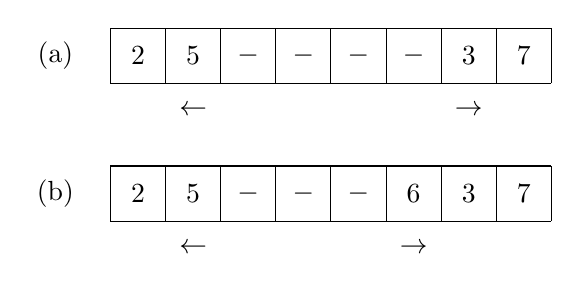
\begin{tikzpicture}[scale=0.7]
\begin{scope}
\draw (0,0) grid (8,1);
\node at (-1,0.5) {(a)};
\node at (0.5,0.5) {$2$};
\node at (1.5,0.5) {$5$};
\node at (2.5,0.5) {$-$};
\node at (3.5,0.5) {$-$};
\node at (4.5,0.5) {$-$};
\node at (5.5,0.5) {$-$};
\node at (6.5,0.5) {$3$};
\node at (7.5,0.5) {$7$};
\node at (1.5,-0.5) {$\leftarrow$};
\node at (6.5,-0.5) {$\rightarrow$};
\end{scope}
\begin{scope}[yshift=-2.5cm]
\draw (0,0) grid (8,1);
\node at (-1,0.5) {(b)};
\node at (0.5,0.5) {$2$};
\node at (1.5,0.5) {$5$};
\node at (2.5,0.5) {$-$};
\node at (3.5,0.5) {$-$};
\node at (4.5,0.5) {$-$};
\node at (5.5,0.5) {$6$};
\node at (6.5,0.5) {$3$};
\node at (7.5,0.5) {$7$};
\node at (1.5,-0.5) {$\leftarrow$};
\node at (5.5,-0.5) {$\rightarrow$};
\end{scope}
\end{tikzpicture}
\caption{(a) Lista $[3,7,2,5]$ tallennettuna taulukkoon. (b) Listan alkuun lisätään alkio 6.}
\label{fig:lismol}
\end{figure}


\subsection{Javan rakenteet}

Javassa \texttt{ArrayList}-rakenne toteuttaa taulukkolistan,
jossa on nopeaa lisätä alkio loppuun sekä poistaa alkio lopusta.
Esimerkiksi seuraava koodi luo listan, lisää siihen alkiot
1, 2 ja 3 ja tulostaa listan sisällön.
Sitten koodi poistaa listan viimeisen alkion ja
tulostaa uudestaan listan sisällön.

\begin{code}
ArrayList<Integer> lista = new ArrayList<>();
lista.add(1);
lista.add(2);
lista.add(3);
System.out.println(lista); // [1, 2, 3]
lista.remove(2);
System.out.println(lista); // [1, 2]
\end{code}

Metodit \texttt{add} ja \texttt{remove}
toimivat keskimäärin ajassa $O(1)$,
joten voimme muuttaa tehokkaasti listaa sen lopusta.
Lisäksi koska lista on tallennetu taulukkona,
voimme tehokkaasti hakea tietyssä kohdassa olevan alkion
ja muuttaa tietyssä kohdassa olevaa alkiota
metodeilla \texttt{get} ja \texttt{set}.

Javassa on myös \texttt{ArrayDeque}-rakenne,
joka toteuttaa taulukkolistan, johon voi tehdä tehokkaita
lisäyksiä ja poistoja sekä alussa että lopussa.
Seuraava koodi esittelee rakenteen käyttämistä:

\begin{code}
ArrayDeque<Integer> lista = new ArrayDeque<>();
lista.addLast(1);
lista.addFirst(2);
lista.addLast(3);
System.out.println(lista); // [2, 1, 3]
lista.removeFirst();
System.out.println(lista); // [1, 3]
\end{code}

\texttt{ArrayDeque} sisältää metodit \texttt{getFirst} ja
\texttt{getLast}, joiden avulla voimme hakea listan
ensimmäisen ja viimeisen alkion.
Kuitenkaan rakenteessa ei ole yleistä metodia \texttt{get},
joten emme pysty hakemaan muita listalla olevia alkioita.

\section{Linkitetty lista}

Linkitetty lista muodostuu solmuista, joista jokainen sisältää
yhden listan luvun.
Solmut on yhdistetty toisiinsa yleensä niin,
että jokaisessa solmussa on viittaus seuraavaan ja
edelliseen solmuun listassa.
Tämän ansiosta voimme esimerkiksi käydä listan läpi ensimmäisestä
solmusta alkaen.

Kuvassa X on esimerkkinä linkitetty lista,
joka vastaa listaa $[3,7,2,5]$.

Taulukkolistaan verrattuna linkitetyn listan etuna on,
että voimme lisätä alkion mihin tahansa kohtaan listaa
$O(1)$-ajassa: riittää luoda yksi solmu ja muuttaa paria
viittausta.
Samoin voimme poistaa minkä tahansa solmun $O(1)$-ajassa.
Huonona puolena on kuitenkin, että tietyssä kohdassa listaa
olevan alkion käsittely vie aikaa $O(n)$: meidän täytyy
kulkea alkioon askel kerrallaan listan alusta tai lopusta.

\subsection{Linkitetyt rakenteet}

Jokaisessa ohjelmointikielessä on omat keinonsa
linkitetyn rakenteen toteuttamiseen.
Javassa voimme toteuttaa linkitetyn rakenteen niin,
että jokainen solmu on oma olionsa.
Esimerkiksi voimme toteuttaa seuraavan luokan \texttt{Node},
jonka oliot toimivat linkitetyn listan solmuina:

\begin{code}
public class Node {
    public int value;
    public Node next;
    public Node prev;
}
\end{code}

Ideana on, että kenttä \texttt{value} kertoo solmun arvon,
kenttä \texttt{next} osoittaa seuraavaan solmuun
ja kenttä \texttt{prev} osoittaa edelliseen solmuun.
Jos seuraavaa tai edellistä solmua ei ole,
viittauksen tilalla on arvo \texttt{null}.
Tämän luokan avulla voisimme luoda linkitetyn listan $[3,7,2,5]$
seuraavasti:

\begin{code}
Node s1, s2, s3, s4;
s1.value = 3; s1.prev = null; s1.next = s2;
s2.value = 7; s2.prev = s1; s2.next = s3;
s3.value = 2; s3.prev = s2; s3.next = s4;
s4.value = 5; s4.prev = s3; s4.next = null;
\end{code}

Tämän jälkeen voisimme käydä listan läpi näin:

\begin{code}
Node s = s1;
while (s != null) {
    System.out.println(s.value);
    s = s.next;
}
\end{code}

\subsection{\texttt{LinkedList}-rakenne}

Käytännössä meidän ei kuitenkaan tarvitse toteuttaa
linkitettyä listaa itse Javalla,
koska voimme käyttää valmista \texttt{LinkedList}-rakennetta.
Voimme lisätä ja poistaa alkioita $O(1)$-ajassa
sekä listan alussa että lopussa.

\begin{code}
LinkedList<Integer> lista = new LinkedList<>();
lista.addLast(1);
lista.addFirst(2);
lista.addLast(3);
System.out.println(lista); // [2,1,3]
lista.removeFirst();
System.out.println(lista); // [1,3]
\end{code}

TODO listan muuttaminen

\texttt{LinkedList} tarjoaa myös metodit \texttt{get} ja \texttt{set},
joiden avulla voi käsitellä tietyssä kohdassa listaa olevaa alkiota.
Näiden metodien aikavaativuus on kuitenkin $O(n)$,
eli \texttt{LinkedList} ei ole hyvä valinta,
jos meidän täytyy käsitellä alkioita kohdan perusteella.

\subsection{Tehokkuusvertailu}

Jokaisessa tietorakenteessa on omat hyvät ja huonot puolensa,
ja kaikille on tietyt käyttötarkoituksensa.
Linkitetty lista muodostaa kuitenkin poikkeuksen tähän sääntöön:
on äärimmäisen harvoja tilanteita, jolloin sitä kannattaisi
käyttää taulukkolistan sijasta.

\begin{figure}
\center
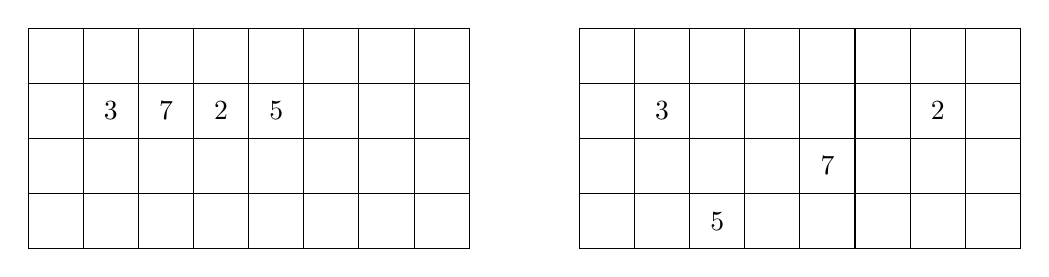
\begin{tikzpicture}[scale=0.7]
\begin{scope}
\draw (0,0) grid (8,4);
\node at (1.5,2.5) {3};
\node at (2.5,2.5) {7};
\node at (3.5,2.5) {2};
\node at (4.5,2.5) {5};
\end{scope}
\begin{scope}[xshift=10cm]
\draw (0,0) grid (8,4);
\node at (1.5,2.5) {3};
\node at (4.5,1.5) {7};
\node at (6.5,2.5) {2};
\node at (2.5,0.5) {5};
\end{scope}
\end{tikzpicture}
\caption{Taulukkolista ja linkitetty lista tietokoneen muistissa.}
\label{fig:taulin}
\end{figure}


Syynä tähän on, että nykyaikaiset tietokoneet on suunniteltu niin,
että ne \emph{suosivat} taulukkolistan käyttämistä linkitetyn
listan sijaan.
Kuvassa \ref{fig:taulin} näkyy, miten taulukkolista ja linkitetty lista
asettuvat tietokoneen muistissa.
Taulukkolistan alkiot ovat peräkkäin, kun taas linkitetyn
listan alkiot voivat olla eri puolilla muistia sekalaisessa
järjestyksessä.
Nykyaikaisen prosessorin välimuistit ja komentojen ennustus
on toteutettu niin, että ne ovat parhaimmillaan silloin,
kun tieto on tallennettu muistissa peräkkäin -- eli juuri kuten
taulukkolistassa.
Tämä näkyy käytännössä siinä, että taulukkolistan käsittely on selvästi
nopeampaa kuin linkitetyn listan käsittely.

Tarkastellaan esimerkkinä seuraavaa metodia,
joka laskee listan lukujen summan.
Koska metodi on toteutettu tyypille \texttt{List},
voimme käyttää sitä sekä tyypin \texttt{ArrayList}
että \texttt{LinkedList} kanssa.

\begin{code}
long summa(List lista) {
    long s = 0;
    for (Integer x : lista) {
        s += x;
    }
    return s;
}
\end{code}
